\documentclass[12pt,letterpaper]{article}
\usepackage[latin1]{inputenc}
\usepackage{amsmath}
\usepackage{amsfonts}
\usepackage{amssymb}

% the above packages are the "base"

\usepackage{graphicx}
\graphicspath{{../figs/}} % set the location of your figures

\usepackage{hyperref} % enable links within pdf
\hypersetup{colorlinks = true, linkcolor = black, urlcolor = blue}


\usepackage{parskip}
\usepackage{pdfpages} % enable insertion of another pdf

\usepackage{bm}
\usepackage{xcolor}


\setcounter{secnumdepth}{0}  % don't number sections (stars not needed)


%\author{Mark Novak}
\title{Getting starting with \texttt{Git}}

\begin{document}
\maketitle

\tableofcontents

\pagebreak


\section{What is version control?}
Version control software allows you to save and provide meta-information on any and all changes you make to a set of files and directories.  It allows you to more easily document changes and the evolution of your files, find and correct bugs that have crept into your code, and revert back to old file versions when needed.  By using version control you'll now what, when and (hopefully) why changes were made.  If you're using the software collaboratively, you'll also know by whom changes were made.  Backing-up is virtually implicit (though not totally so), especially when you also use a networked (off-site) server as a host for your repository.

We'll be using \texttt{Git} as our version control software.  There are others out there (e.g., \texttt{Subversion}).  We'll also be using \texttt{Github} as our host.  There are others out there (e.g., \texttt{Bitbucket}).

\section{Git}
\texttt{Git} was developed by Linus Torvalds (the ``Linu'' in Linux).  Most of its features are accessed by command-line and are intended for large-scale collaborative programming and software development purposes.  Of course, we'll be using \texttt{Git} for much smaller, specific projects, thus we won't bother with many of these feature.  We'll also interact with \texttt{Git} using GUIs (e.g., \texttt{R-Studio}) rather than command-line.

\textbf{Required reading} to get an overview of how \texttt{Git} works:\\
\begin{footnotesize}
  \url{https://git-scm.com/book/en/v2/Getting-Started-What-is-Git%3F}.
\end{footnotesize}

\section{Github}
\texttt{Git} enables you to store a complete copy of the project on your local machine, including its history and all versions.  That means that no centralized server is necessary.  However, if you want to collaborate with others, have multiple computers with which you'd like to work, or want to create true back-ups of your project, then you'll also want to use a server on which to host your repository.  Fortunately, there are a number of free providers.

For \texttt{Git}, the primary options are \texttt{Github} and \texttt{Bitbucket}.  The former is more developed (more bells and whistles), is currently more widely used, and is perhaps a little easier to work with.  The two don't differ all that much except in one regard:  the number of free versus public repositories.  While \texttt{Github} has a limit on the number of private repositories, \texttt{Bitbucket} has a limit on the number of collaborative projects (having more than 5 collaborators).  (There may still be perks regarding the number of repositories when you sign up using an academic email address.  See \url{https://help.github.com/en/articles/applying-for-an-educator-or-researcher-discount})

\textbf{To do:} Create an account on \texttt{github}.  (I suggest creating accounts with both hosts.  I use them for different projects, as needed.)


\section{Installing and configuring Git}
To install and configure \texttt{Git} on a PC, go see \\
\url{https://git-scm.com/book/en/v2/Getting-Started-Installing-Git}

To install \texttt{Git} on a Mac:

\url{http://code.google.com/p/git-osx-installer}\\
or\\
\url{http://git-scm.com/downloads}


After you install \texttt{Git} there's a little (minimum of) command-line configuration to perform.  On a Mac, open a \texttt{Terminal} window and type in the following:

     \texttt{\$ git config --global user.name "Mark Novak"}\\
     \texttt{\$ git config --global user.email "Mark.Novak@oregonstate.edu"}

Some of you might want to set up an editor to be used in git, for example:

	\texttt{\$ git config --global core.editor emacs}

You can check to ensure that these commands when through and see what other things you might want to configure using

	\texttt{\$ git config --list}

For more, see\\
\begin{footnotesize}
\url{https://git-scm.com/book/en/v2/Getting-Started-First-Time-Git-Setup}
\end{footnotesize}

\section{Repository setup}
There are command-line methods for doing everything we're going to do below.  Indeed, command-line is the default way that most people interact with \texttt{Git}. (See last page for a cheat sheet.)  Instead, we're going to make use of the tools made available through \texttt{Github}, starting with the very first step of initiating a repository and getting some minimal information associated with it.  That is, rather than creating and setting up a repository on our computer by command-line and then connecting it to \texttt{Github}, we'll create and set it up on \texttt{Github} and clone it to our local  master folder of projects.

Simply log in to your \texttt{Github} account, click on ``New Repository'', and follow the instructions.  These should include options for private versus public (pick the latter for this class), initializing with a \texttt{README} file (which you \emph{should} do), and adding a \texttt{.gitignore} file (which you \emph{should} also do).

The \texttt{README} file is the first file that anyone will look at when they inspect your repository (assuming it's public).  It should give an overview of what the project is about and what the various parts of the project structure are.  We will learn to use Markdown to write and edit README files later in the course, so for now put some minimally useful text in it without any formatting (e.g., your project title).

The \texttt{.gitignore} file contains a list of all the files that you want \texttt{Git} to ignore (not monitor for changes).  Selecting \texttt{R} from the dropdown list will auto-fill a bunch of it for you.  Later in the course we'll also add the extensions for all the temporary files that \LaTeX produces when compiling.

You should now see a new webpage -- your Repo page -- that shows you what's in your repository.  For now it contains only the  \texttt{.gitignore} and \texttt{README.md} files, the latter of which has its contents displayed.  As I said earlier, there's a lot of bells-and-whistles at your fingertips here (the most useful of which for collaborative projects is the \texttt{Issues} feature).  You \emph{could} start dragging-in directories and files to add them to your repository, but we're \emph{not} going to do that.  Instead, we're going to \texttt{clone} this repository to our local machine, then add our various project sub-folders to it (from your projectfolder) and go from there.

To clone the repository, click the green \texttt{Clone or download} button and copy the provided URL.

Now there's a couple ways to clone your repository to your local machine.  The preferred method depends on how you're most likely going to interface with \texttt{Git}.  You could:
\begin{enumerate}
	\item use command-line to clone.  Open \texttt{Terminal}, \texttt{cd} into your \texttt{Projects} master folder, then type \texttt{git clone} followed by the URL;
	\item use a visual \texttt{Git} GUI client to clone the repo;
	or, if you're going to be primarily using \texttt{R} via \texttt{R-Studio} anway,
	\item set up a ``project'' within \texttt{R-Studio} first and provide it with the URL during setup.  It'll then clone the repo for you.
\end{enumerate}

\section{R-Studio and Git GUIs}
I use \texttt{Git} for both \texttt{R} and non-\texttt{R} (e.g.,  \texttt{Mathematica})-based projects.  Only  \texttt{R-Studio} has integrated  \texttt{Git} functionality, so I use a visual  \texttt{Git} GUI client (e.g., \texttt{Sourcetree}) for some projects because I can't be bothered to memorize the  \texttt{Git} command-line commands.  Since most of you are probably using \texttt{R}, it's probably worthwhile to use \texttt{R-Studio}'s  \texttt{Git} integration feature (which is the only reason I use  \texttt{R-Studio} to begin with).

You'll first need to tell  \texttt{R-Studio} that you have \texttt{Git} installed, so go to its Preferences, select \texttt{Git/SVN} and fill in the details: either click on the Help link or go to
\url{http://r-pkgs.had.co.nz/git.html} to see what to do.

Now create your ``project'' within  \texttt{R-Studio} by selecting ``New Project''.  Select \texttt{Version Control: Checkout a project from...repository}, select \texttt{Git}, and fill in the details including the URL you got from \texttt{Github}.  The directory in which you place your repository should be your master folder.   \texttt{R-Studio} will ``restart'' and then you'll be in your project (as evidenced by its name appearing in the top-right of the interface).  Clicking on the \texttt{Files} tab will show you what's in the repository (which should at present be: \texttt{README.md}, \texttt{.gitignore} and the newly created \texttt{.Rproj} file).

You may now create (or move in) all your project sub-folders.


\section{Git work flow}
First, \textbf{required reading:}\\
\url{https://git-scm.com/book/en/v2/Getting-Started-What-is-Git%3F}

Basically, files (or directories) exist in one of four states of a life-cycle: untracked, staged, unmodified, or modified (see Fig. \ref{fig:lifecycle}).  The standard workflow is thus:
\begin{enumerate}
	\item Add or modify some files.
	\item Stage the new or modified files.
	\item Commit the changes (moving them from the Staging Area to the ``memory'' of the repository).
	\item Repeat.
\end{enumerate}

\begin{figure}
	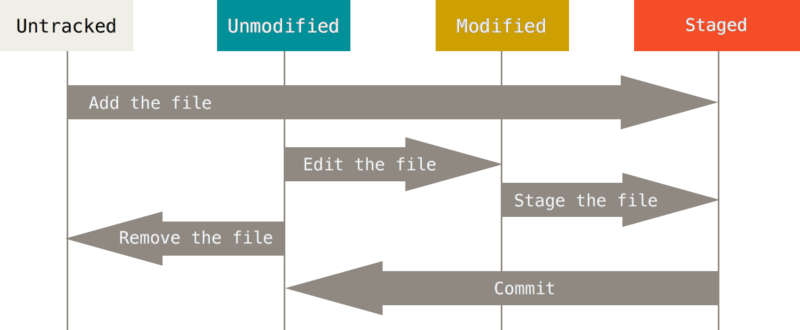
\includegraphics[width=\linewidth]{lifecycle.png}
	\caption{The \texttt{Git} life-cycle.}
	\label{fig:lifecycle}
\end{figure}

The motto of \texttt{Git} is ``\emph{commit early, commit often}''.  Every time you add or remove something from your project (i.e. a file or a chunk of code), you want to commit those changes.   Ideally, each commit should correspond to a ``logical unit'', one that you are able to describe in a few words (e.g., ``function to perform resampling added to analysis script''). Choosing when to commit is quite important, especially when you're debugging code:  For example, if you've discovered your code has two bugs then you should commit each one of the fixes seperately, not together.  That way you can undo either fix independently if, for example, you messed up in one of your fixes or your fix created a different bug somewhere else in your code.

Within \texttt{R-Studio} (and assuming you have your \texttt{R-Studio} project opened), looking at the \texttt{Git} tab will show you a list of all the files (and directories) that have been changed, removed or added to the project since the last time you committed.  Clicking on the check-boxes associated with each file will add them to the staging area.  Clicking on \texttt{Diff} or \texttt{Commit} will open up a new interface (the staging area).  In the top-left corner you'll see a list of the staged files.  Selecting one of the files will bring its contents up in the window below which highlights the text that has been added (in green) and removed (in red).  Select all the files you want to commit, then add a commit message to the top-right window, and commit.

You've now updated your local respository.  Clicking on \texttt{History} (top-left) will show you all your past commits.  Remember, ``\emph{commit early, commit often}''.


\begin{figure}
	\centering
	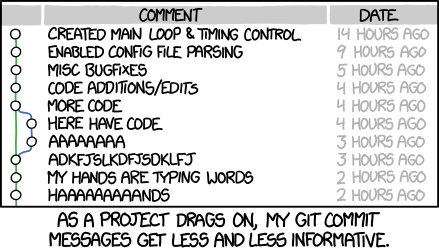
\includegraphics[width=0.5\linewidth]{xkcd_git_commit.png}
	\caption{Don't let this happen!  (source: \url{http://xkcd.com/1296/})}
	\label{fig:commit_messages}
\end{figure}

The final thing to do (often, for back-up reasons, but not necessarily following each commit) is to \texttt{Push} your commit to \texttt{Github}.  \texttt{Pull} obviously does the opposite: bringing commits that have been saved to \texttt{Github} (by others, or by you on a different machine) to your local machine.

\emph{ \textbf{Note:}  To avoid conflicts, the safe thing to do is to always pull before you start making edits, commit and push.  There are of course ways of dealing with conflicts and merging files (that will arise if two people are working on the same file, for example), but for our mostly single-user purposes it's easier to just avoid them.}


\section{Git resources}
There's a whole lot more functionality to \texttt{Git}, some of which is important and very useful (such as resolving conflicts, branching and merging, and reverting back to old versions), but we're not going to get into that unless we have extra time.  For more information, check out the following resources:

\url{https://www.codecademy.com/learn/learn-git}\\
\url{https://www.atlassian.com/git/tutorials}\\
\url{http://rogerdudler.github.io/git-guide/}\\
\url{https://git-scm.com/book/en/v2}



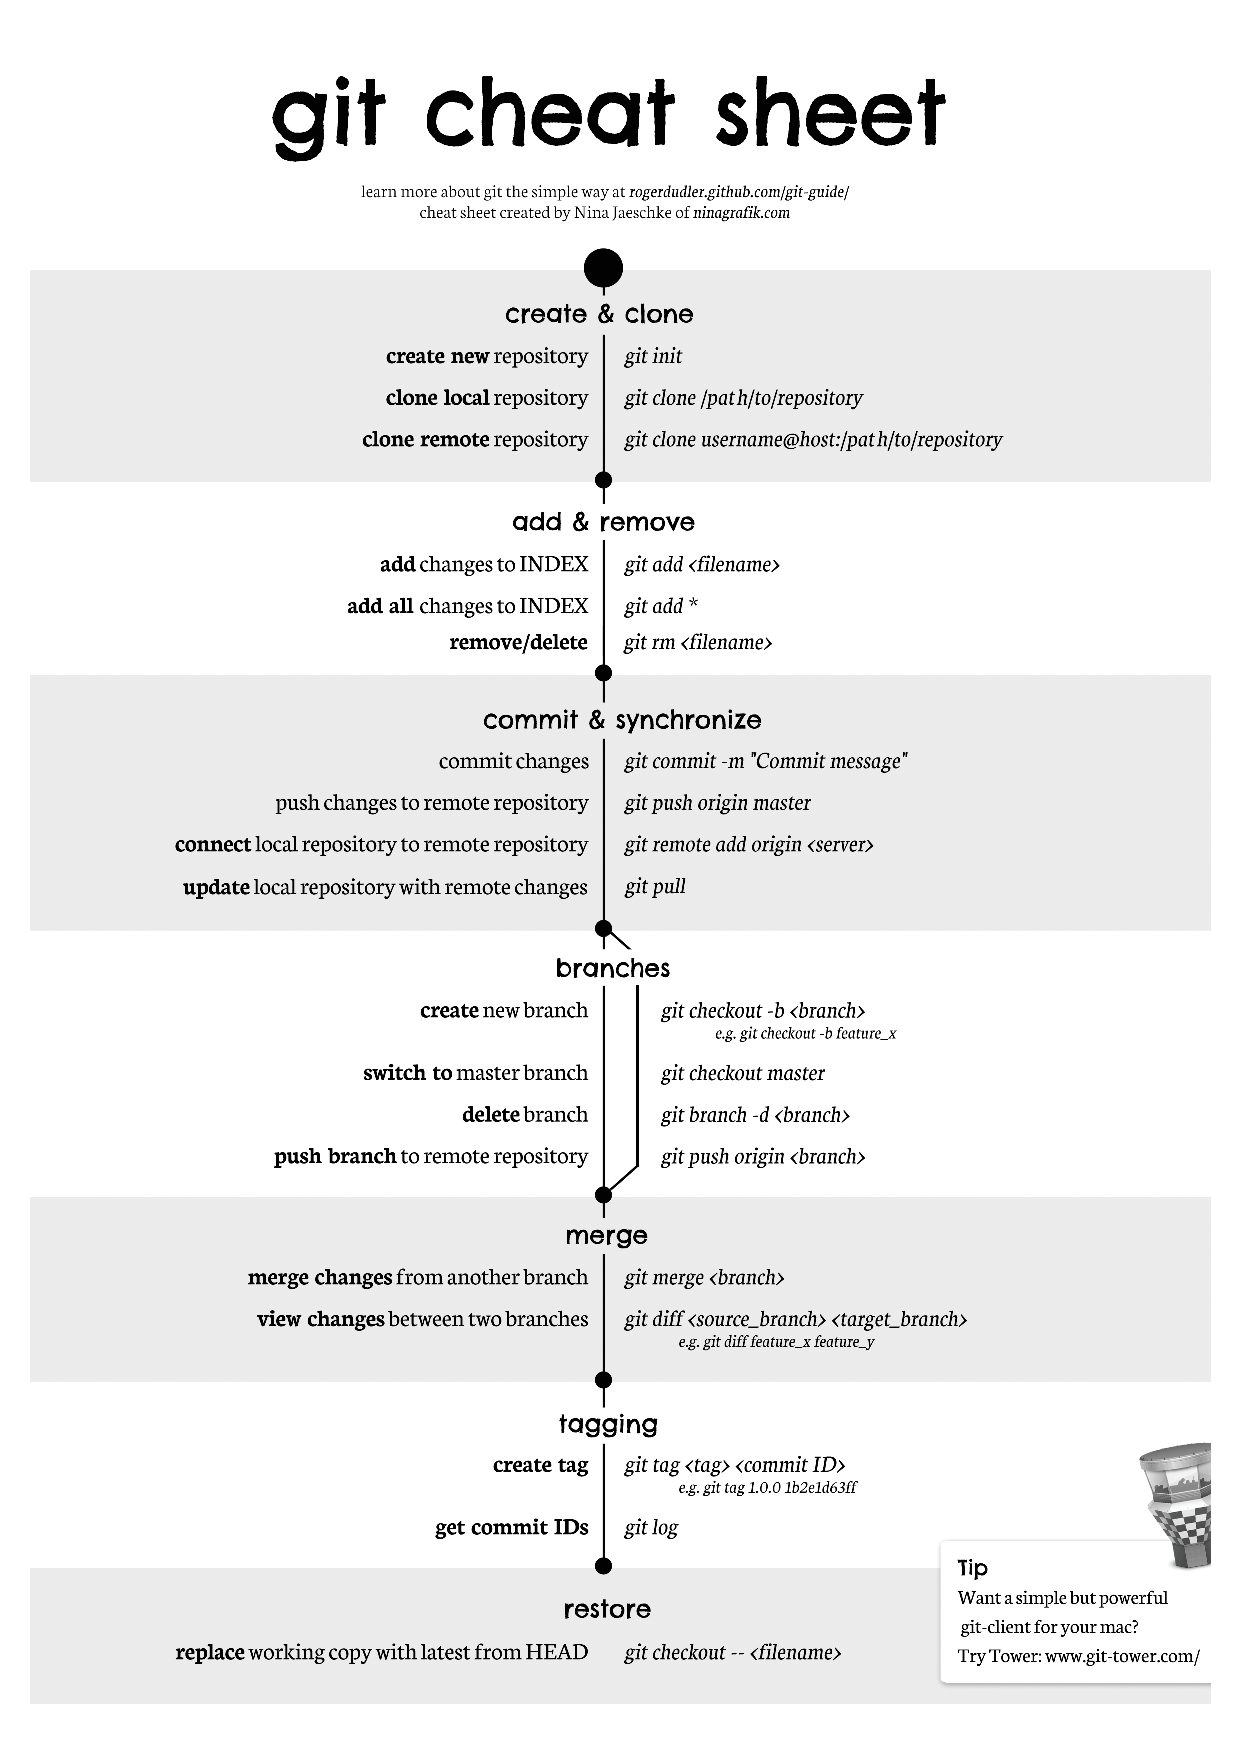
\includepdf{../reference/git_cheat_sheet.pdf}

\end{document}
